\chapter{Methoden} \label{chap:methoden}

\section{Phylogenetische Analyse} \label{sec:phylogenetische-analyse}

Für die phylogenetische Untersuchung der Flaviviridae-Familie wurden 458 vollständige Genomsequenzen aus öffentlichen Datenbanken wie GenBank extrahiert und sorgfältig kuratiert, um eine hohe Datenqualität sicherzustellen \autocite{mifsudMappingGlycoproteinStructure2024}. Als phylogenetischer Marker diente das \gls{nsfive}-Gen, welches die RNA-abhängige RNA-Polymerase (\gls{rdrp}) kodiert und aufgrund seiner hohen Konservierung ideal für solche Analysen geeignet ist \autocite{Koonin1991}.

Die ausgerichteten Sequenzen wurden mithilfe des Programms \gls{mafft} zu einem Multiplen Sequenzalignment (\gls{msa}) verarbeitet \autocite{Katoh2013}. Dabei kombiniert MAFFT effiziente Algorithmen mit Fourier-Transformationen, um konservierte und variable Regionen innerhalb der Sequenzen präzise zu identifizieren. Die mathematischen Details der Fourier-Transformation in diesem Zusammenhang finden sich im Anhang \ref{sec:mafft-mathematik}.

Anschließend wurde das resultierende \gls{msa} für die Rekonstruktion eines phylogenetischen Baumes verwendet, der mithilfe der Maximum-Likelihood-Methode und dem Substitutionsmodell \gls{gtrig} erstellt wurde. Die mathematische Formulierung der Maximum-Likelihood-Methode und des \gls{gtrig}-Modells ist im Anhang \ref{sec:maxlikelihood} näher erläutert. Dieses Modell erlaubt eine flexible Modellierung von Nukleotidsubstitutionen und ist besonders für komplexe phylogenetische Beziehungen geeignet \autocite{Tavare1986}.

Die Robustheit der rekonstruierten Topologie wurde durch Bootstrapping mit 1.000 Wiederholungen getestet, um die statistische Unterstützung der Knoten zu evaluieren \autocite{Felsenstein1985}. Hohe Bootstrap-Werte bestätigen die Zuverlässigkeit der wichtigsten evolutionären Abzweigungen und ermöglichen eine detaillierte Klassifizierung der Hauptkladen innerhalb der Flaviviridae. Weitere Details zur Berechnung des Bootstrappings sind ebenfalls im Anhang \ref{sec:maxlikelihood} beschrieben.

\section{Proteinstrukturvorhersage: ColabFold und ESMFold} \label{sec:colabfold-esmfold}

Die dreidimensionalen Strukturen der Glycoproteine der Flaviviridae wurden mithilfe von \gls{colabfold} und \gls{esmfold} vorhergesagt. Beide Methoden basieren auf tiefen neuronalen Netzwerken, unterscheiden sich jedoch im Ansatz und ergänzen sich ideal.

\gls{colabfold}, eine optimierte Implementierung von AlphaFold2, kombiniert Multiple Sequence Alignments (\glspl{msa}) mit Transformer-Netzwerken, um präzise Strukturvorhersagen zu liefern \autocite{Mirdita2022}. Zunächst werden homologe Sequenzen aus großen Datenbanken wie \gls{uniref} und \gls{bfd} identifiziert und in einem MSA zusammengefasst. Die daraus extrahierten evolutionären Informationen werden im Evoformer-Modul verarbeitet, um langreichweitige Wechselwirkungen zwischen Aminosäuren zu modellieren. Abschließend erfolgt die Vorhersage der Proteinstruktur, deren Qualität mithilfe der \gls{plddt}-Werte bewertet wird.

Die mathematische Formulierung der pLDDT-Werte und die Berechnung der Root-Mean-Square Deviation (\gls{rmsd}) zur Bewertung der Strukturen sind im Anhang \ref{sec:rmsd-berechnung} näher beschrieben.

\begin{figure}[H]
    \centering
    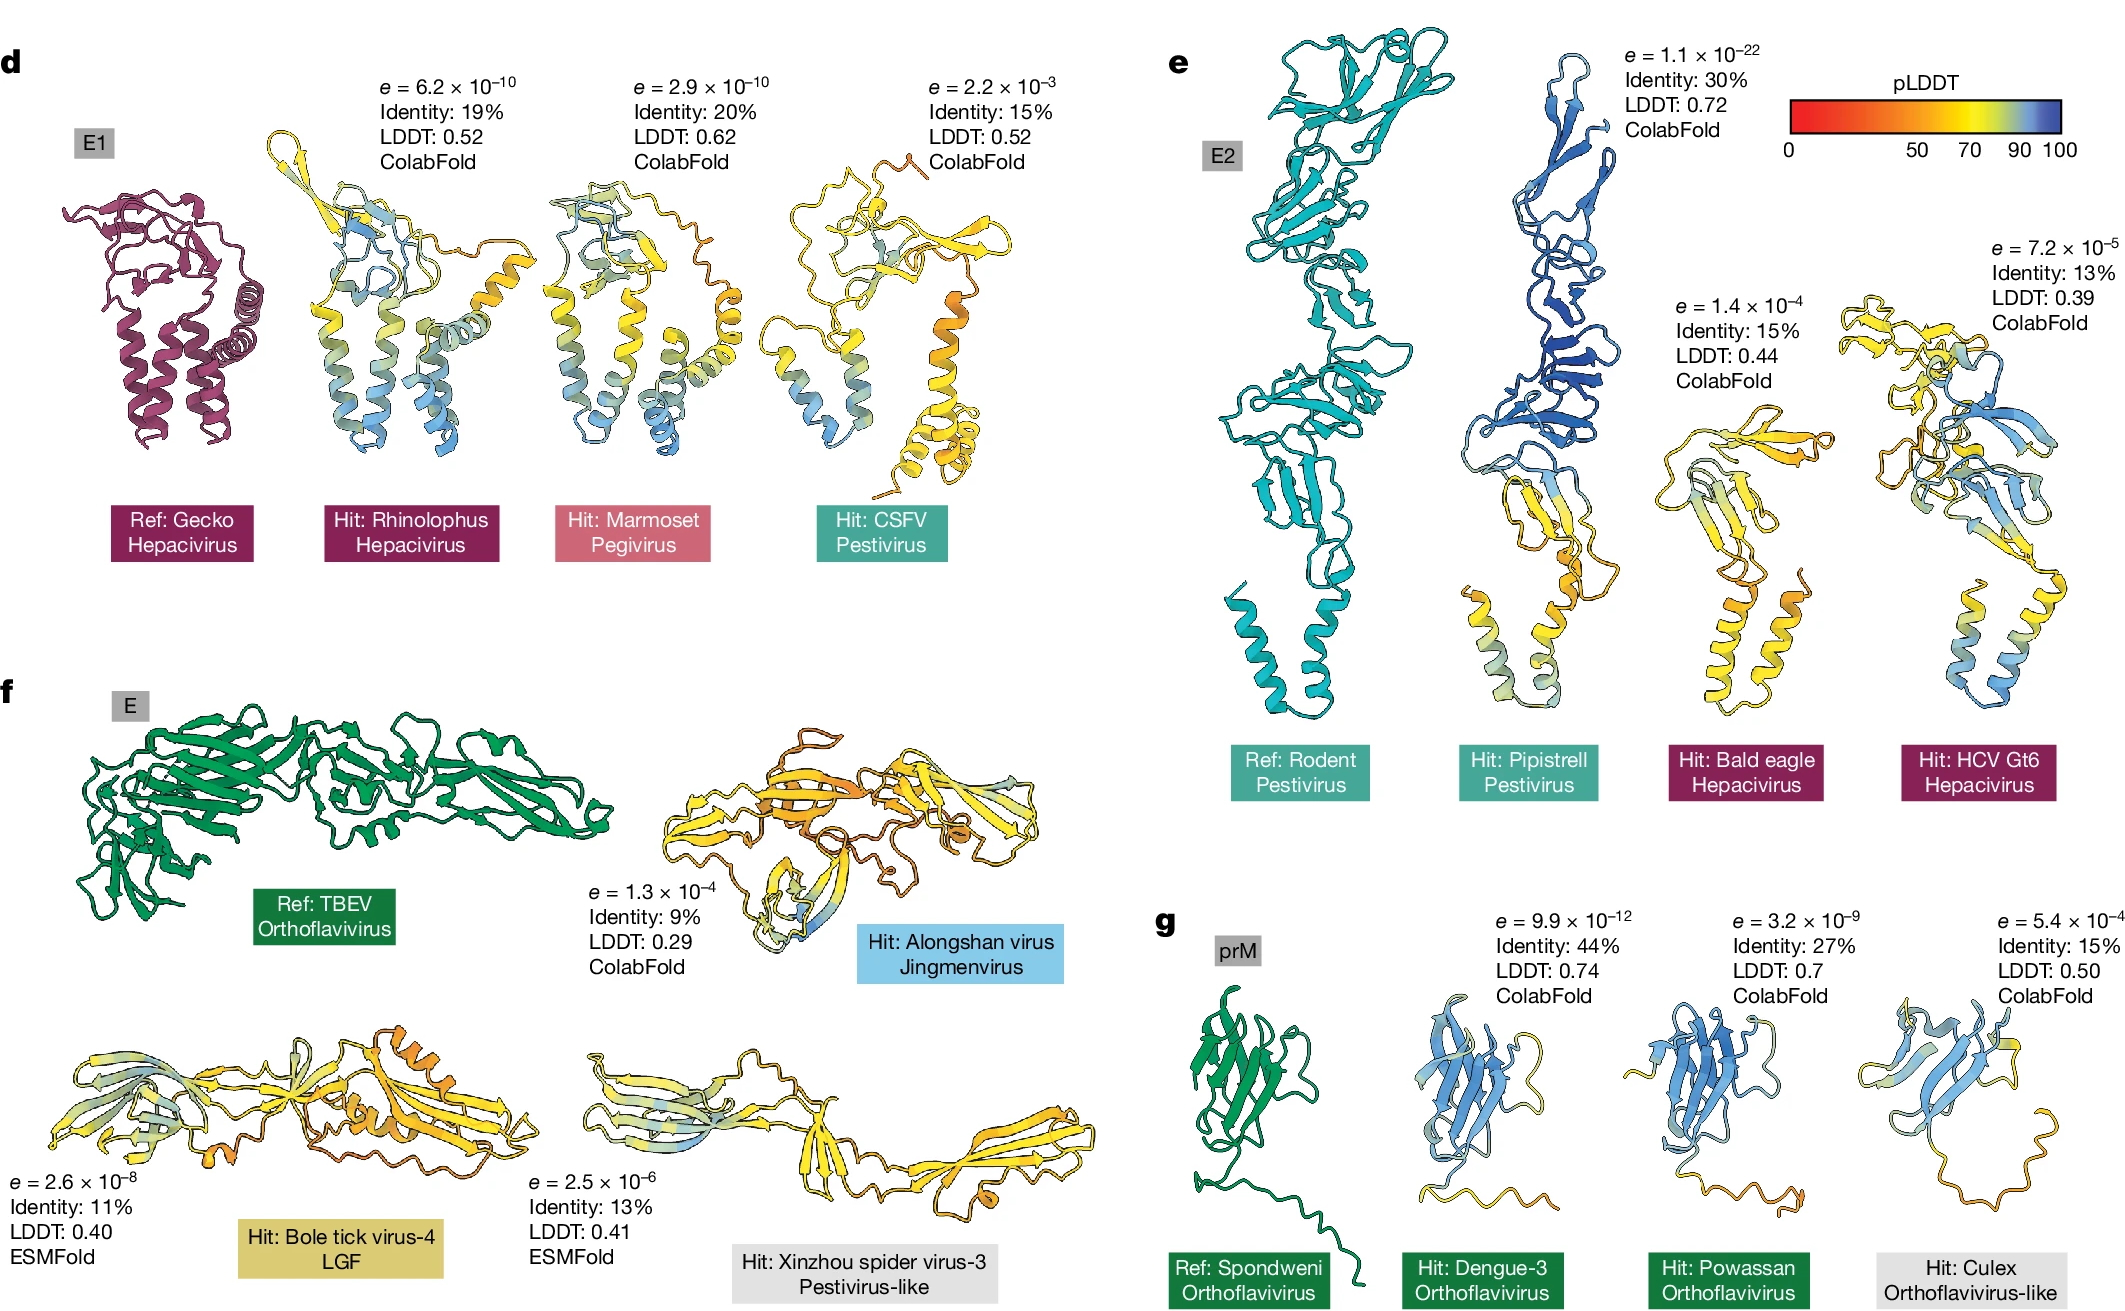
\includegraphics[width=.9\textwidth]{/workspaces/seminar-bioinformatik/images/figure2.jpg}
    \caption{Illustration der pLDDT-Werte in Korrelation mit den \gls{msa}-Alignments}
    \label{fig:figure2-orginal}
\end{figure}

Im Gegensatz dazu verwendet \gls{esmfold} einen sprachmodellbasierten Ansatz, der keine \glspl{msa} benötigt. Hierbei wird die Proteinsequenz direkt durch ein Transformer-Sprachmodell analysiert, das auf Millionen von Sequenzen trainiert wurde \autocite{linEvolutionaryscalePredictionAtomiclevel2023}. Besonders bei hochdivergenten Proteinen mit wenigen homologen Sequenzen liefert ESMFold zuverlässige Ergebnisse, indem es die Sequenzinformationen kontextabhängig interpretiert.

\section{Homologiesuche: Anwendung von Foldseek} \label{sec:foldseek}

Zur Identifizierung struktureller Homologien zwischen den vorhergesagten Glycoprotein-Strukturen wurde das Programm \gls{foldseek} eingesetzt \autocite{vankempenFastAccurateProtein2024}. Foldseek ermöglicht einen schnellen Vergleich von Proteinstrukturen, indem es deren dreidimensionale Koordinaten in vereinfachte Merkmalsrepräsentationen umwandelt. Diese Methode ist besonders effizient, um strukturelle Ähnlichkeiten auch bei hoher Sequenzdivergenz zu erkennen, was klassische sequenzbasierte Methoden wie BLAST nicht leisten können \autocite{Altschul1990}.

Die vorhergesagten Glycoprotein-Strukturen aus \gls{colabfold} und \gls{esmfold} wurden mit bekannten Strukturen aus der Protein Data Bank (\gls{pdb}) verglichen. Die Übereinstimmung der Modelle wurde durch Alignment-Scores und \gls{rmsd}-Werte quantifiziert, deren mathematische Grundlagen im Anhang \ref{sec:rmsd-berechnung} erläutert werden. Konservierte Faltungsmuster und potenzielle funktionelle Gemeinsamkeiten, wie die Klasse-II-Fusionsproteinfaltung, wurden identifiziert.

Die Ergebnisse der Homologiesuche wurden anschließend mit den phylogenetischen Analysen kombiniert, um divergente und konvergente evolutionäre Anpassungen innerhalb der Flaviviridae zu identifizieren. Auf diese Weise konnten strukturelle Gemeinsamkeiten zwischen verschiedenen Gattungen trotz erheblicher Sequenzunterschiede nachgewiesen werden.